%!TEX root = ../main.tex
\doublespacing
\chapter{Future Work and Conclusions}
\label{chap:future}
The principle goals of this thesis were to observe solar radio emission at the highest temporal, spectral and spatial resolutions to date. In order to do this, the REAL-time Transient Acquisition backend was developed and installed at I-LOFAR to record the raw voltages fron the station at their native $5.12 \mu$s temporal resolution.
Secondly, a new technique was implemented for the first time to directly measure the size of radio bursts from their interferometric visibilities. This technique was utilised to determine the size and shape of 30 Type III bursts and to compare this with predictions from modern scattering simulations.
This chapter highlights the next steps that can be taken to advance the knowledge of radio wave generation and propagation in the solar corona even further. I discuss the possibility of observing radio bursts with 5 ns temporal resolution using the Transient Buffer Boards from I-LOFAR. I also outline further work that should be done to fully tie together modern observations and computer simulations and the need for a statistical analysis of Type III and Type IIIb radio bursts in order to bring them in line under the most recent theory of Langmuir wave generation. I then draw this thesis to a close with some concluding remarks.

\section{Primary Scientific Objectives}
The research which has been presented in this thesis has contributed to our knowledge of solar radio emission at low frequencies. The extent to which radio wave propagation effects distort the original shape of a radio burst has been narrowed down. Work undertaken during this thesis has also resulted in a new facility to record and analyse radio emission using I-LOFAR. REALTA can be used to record radio observations at 5.12 $\mu$s temporal resolution. A new technique for measuring burst sizes from complex visibility data was also developed over the course of this work and shows promise.

\subsection{Observing Radio Bursts at the Highest Temporal Resolutions.}
In order to record high time resolution data of solar radio bursts from I-LOFAR, a dedicated backend to record, store and analyse the data was necessary. Chapter \ref{chap:instrumentation} outlines the development of REALTA to serve this purpose. The 7 node computer cluster receives data from I-LOFAR along a 10~Gbps fibre optic cable in four data ``lanes". After data has been recorded to disk, one of many processing pipelines can be run including those for solar radio observations, pulsars, FRBs, RRATs, Jovian emission and SETI. Some of the first solar radio bursts observed with I-LOFAR and REALTA are shown in Chapter \ref{chap:instrumentation} while first observations and preliminary results are given in the published version of this work, in \textit{Astronomy and Astrophysics} \citep{Murphy2021b}. Observations of short duration solar radio bursts such as S-bursts can be used to remotely determine the physics of the solar corona \citep{Morosan2015, Clarke2019} while short duration pulsations in radio bursts can give insight into magnetohydrodynamic oscillations in the corona \citep{Carley2019}.

\subsection{Observing Radio Bursts at the Highest Spatial Resolutions.}
In Chapter \ref{chap:measuring_source_sizes} I described a new method for determining the size of Type III radio bursts from LOFAR visibilities. Using this I was able to determine the size of a Type IIIb burst. For a burst at 34.76~MHz, the full width at half maximum height (FWHM) along the major and minor axes was found to be $18.8^\prime$~$\pm~0.1^\prime$ and $10.2^\prime$~$\pm~0.1^\prime$ respectively at a plane of sky heliocentric distance of 1.75~R$_\odot$. The expected size of a burst at this frequency, based on the relationship between the spectral width of the striation and spatial extent of emission, was calculated to be 3.18 arcsec. The discrepancy between these two values was investigated and the results suggest that the level of density fluctuations in the solar corona is the major cause of the scattering of radio waves, resulting in large source sizes. However, because of its inherently lower spatial resolution, the magnitude of $\varepsilon$ may be smaller than previously derived in comparison to observations of radio wave scattering in tied-array images. This work was published in \textit{Astronomy and Astrophysics} as \cite{Murphy2021}.

\subsection{Comparing Observations of Radio Bursts to Computational Simulations.}
Using the new method for determining radio burst size from interferometric visibilities, the spatial properties of 30 Type III radio bursts were found. Chapter \ref{chap:observations_vs_theory} discusses the measured similarities and discrepancies between these observations and computer simulations of scattering. It was found that theories of scattering are unable to account for the distribution of radio burst source sizes if they are intrinsically point sources. The more likely case is that Type III radio bursts have an inherent source size larger than the size due to scattering for a point source. 

\section{Future Work}
The research outlined in this thesis has produced a computationally, and more importantly conceptually, simple method to determine the size and position of a radio burst from its interferometric visibilities. This has been used to bring forward our understanding of radio wave scattering in the solar corona one more incremental step along the vast journey of scientific knowledge. While the current state of REALTA allows for the recording of the raw complex voltages from I-LOFAR to study solar radio bursts, more can be done to automatically determine when a radio burst has occurred in order to save on the ever growing data storage issue. Also, REALTA can be adapted to record data from I-LOFAR's TBBs which can record 5 s of data at the 200/160 MHz sampling of I-LOFAR to give the highest temporal resolution of the Sun recorded in human history. 
 
\subsection{On Observing Radio Bursts with TBBs.}
One of the greatest, unexplored potentials of solar radio astronomy is extremely high temporal resolution of radio bursts. The LOFAR TBBs are capable of recording 5 seconds of raw sampled data from the antennas at its native 5 ns temporal resolution. The TBBs are an extremely powerful tool that allow you to recreate the LOFAR data processing pipeline entirely in software. Typically, the TBB buffer is frozen before all the data is read out to an external disk. This process is much slower than the 3.2 Gbps recording of RSP data and can take upwards of 40 minutes to read out 5 s of data from every TBB. Over the period September 2017 to March 2018 a method of continually reading from the TBBs in almost real time was investigated. The development of such a system was beyond my capabilities from the outset but work by Prof. Brian Coghlan managed to get a working prototype. Unfortunately the goal of a real time readout of TBBs was deemed to be too ambitious for a PhD project and my involvement in that work ended. The data recorded during this time coincided with the solar minimum of solar cycle 24. Radio bursts occurred only once every few months and as such any data taken was essentially noise. Figure \ref{fig:TBB_timeseries} shows 10 ms of noise recorded by the TBBs from LBA number 3 at I-LOFAR.
%
%\begin{figure}[ht]
%\centering
%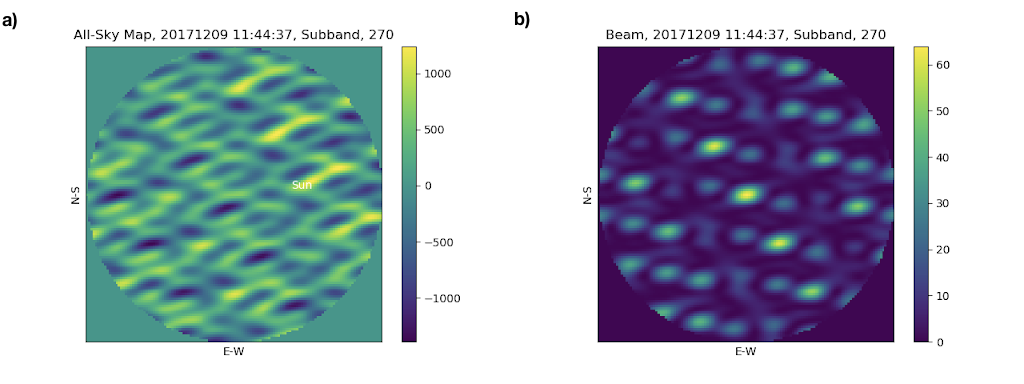
\includegraphics[width=\columnwidth]{AllSky_psf.png}
%\caption[An all sky image made with data from the TBBs at I-LOFAR]{a) An all sky image made with data from the TBBs at I-LOFAR at 52.73 MHz. b) The psf of the antennas for which TBB data was available.}
%\label{fig:TBB_allsky}
%\end{figure}
\begin{figure}[ht]
\centering
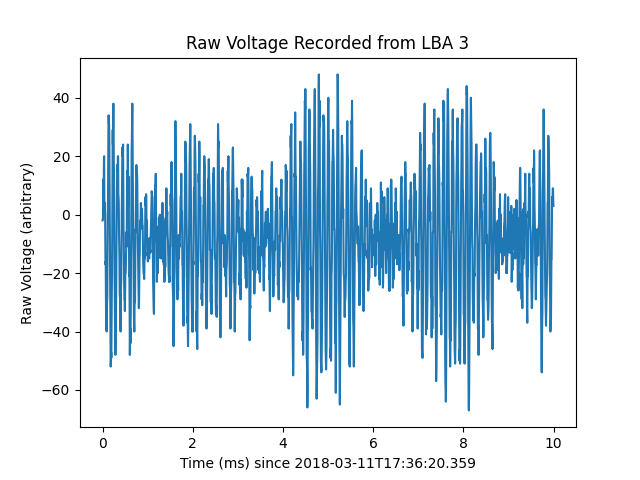
\includegraphics[width=\columnwidth]{TBBtimeseries.png}
\caption[10 ms of data recorded with TBBs from I-LOFAR.]{10 ms of data recorded with TBBs from I-LOFAR, the data presented here is from LBA 3. The beating pattern is likely due to RFI.}
\label{fig:TBB_timeseries}
\end{figure}

The fact that TBB data is recorded before any of the signal processing described in section \ref{sec:sig_pipe} occurs is both a blessing and a curse. It gives you the freedom to recreate a radio telescope from the ground up in software and do some inovative things. Take the follwoing for an example. The polyphase filter bank in an RSP take 1024 time samples before performing a Fourier transform to get 512 subbands. This essentially results in a dynamic spectrum with a temporal resolution of 5.12 $\mu$ s and 192.125 kHz spectral resolution. Using TBB data it is possible to instead, perform an FFT on the entire time series, window the resulting spectrum with any desired frequency resolution and inverse FFT each to get a dynamic spectrum with 5 ns temporal resolution and the chosen spectral resolution. 

\begin{figure}[ht]
\centering
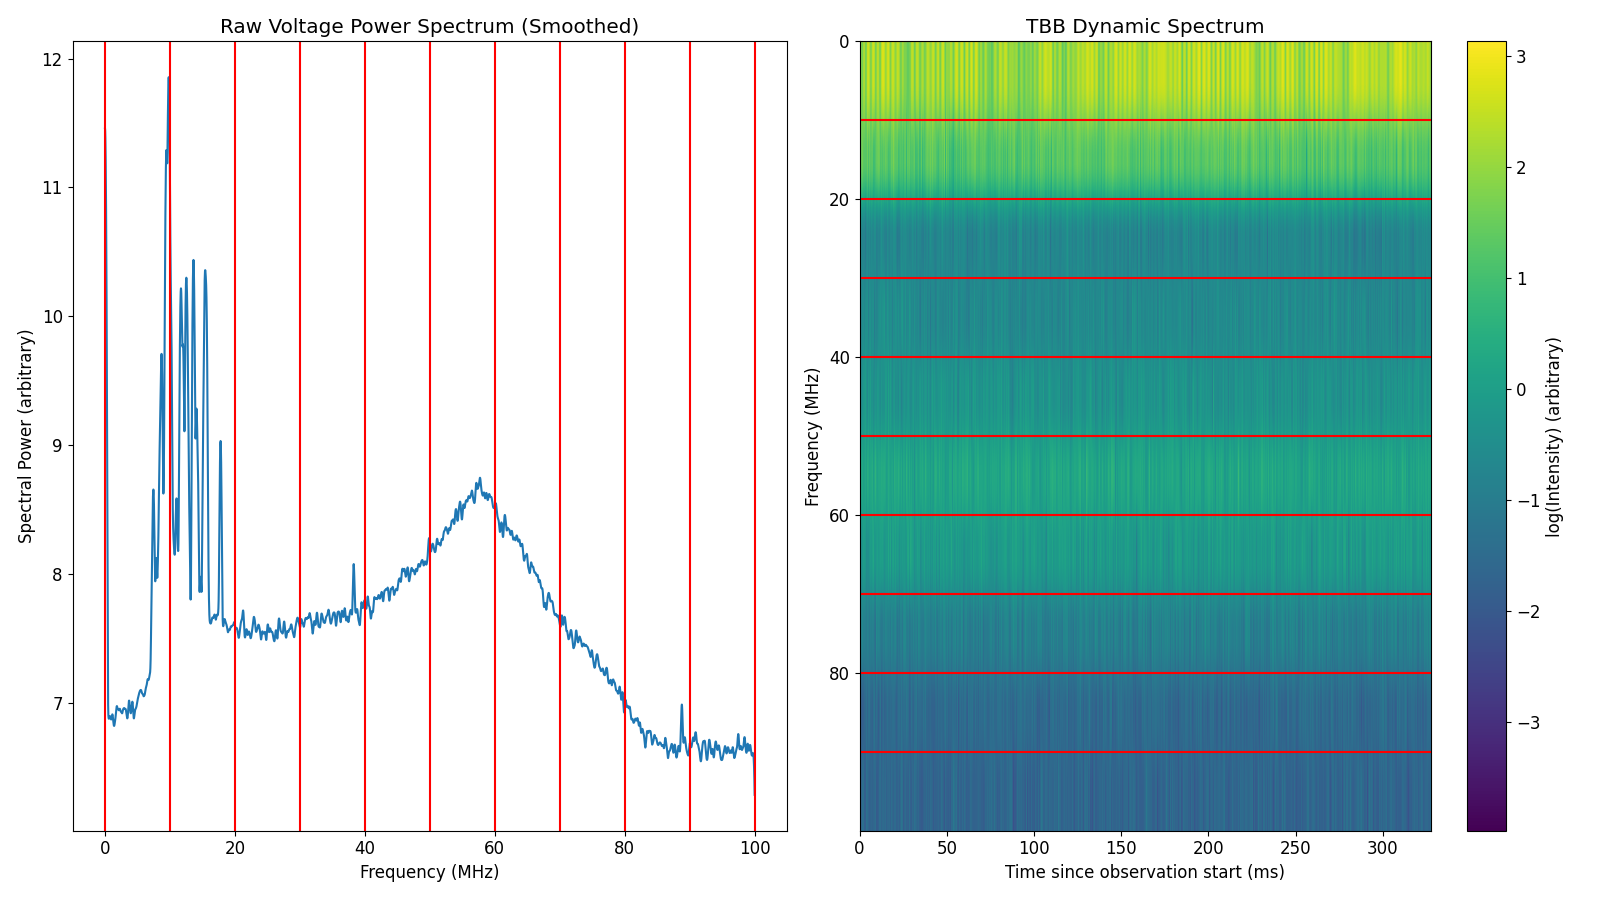
\includegraphics[width=\columnwidth]{TBB_dynamic_spectrum_power_spectrum.png}
\caption[A dynamic spectrum generated with TBB data from I-LOFAR.]{The left panel shows the (smoothed) power spectrum of an LBA. The vertical red lines mark the chosen subband edges. The right panel is a dynamic spectrum with a time resolution of 5ns and frequency resolution of $\sim 10$ MHz as determined by the chosen number of subbands, whose edges are shown by the red horizontal lines.}
\label{fig:TBB_dynamicspectrum}
\end{figure}

Figure \ref{fig:TBB_dynamicspectrum} shows a dynamic spectrum generated from the same TBB data as shown in Figure \ref{fig:TBB_timeseries}. The left panel shows the (smoothed) power spectrum of the time series with a number of vertical red lines which indicate the edges of chosen subbands. By performing an inverse Fourier transform on each subband, a dynamic spectrum with a tmeporal resolution of 5 ns can be created, shown in the right panel where again, the red lines indicate the subband edges. Care must be taken to avoid spectral leakage between subbands although as Figure \ref{fig:TBB_dynamicspectrum} only shows noise, rectangular windows for the subbands are probably good enough.
 
The ability to record dynamic spectra and retain the 5 ns temporal resolution of the raw LOFAR sampling means that, should they exist, extremely short duration pulsations in solar radio bursts could be studied. While it is unlikely that periodic pulsations of the order of 10s of nanoseconds will ever be observed due to the scattering of radio waves in the solar corona, there has been no report in scientific literature of solar radio emission at this time scale and thus, any such study opens the door into the domain of nanosecond observations of the sun.

\subsection{On Automatically Classifying Radio Bursts.}
One of the big challenges facing radio astronomy is the dat produced during observations. I-LOFAR produces 3.2 gigabits of data per second while REALTA only has 5 TB of free storage at any given time. As such, observing the sun for long durations and saving the entire raw data set on the offchance that there is a radio burst is horrifically impractical. An ideal solution would be to automatically determine is a burst has occurred before choosing to save data to disk. \cite{Scully2021} recently showed promising results of using a convolutional neural network (CNN) to automatically detect and characterise Type III radio bursts. They implement the YOLOv2 \citep[You Only Look Once;][]{Yolo9000} algorithm to detect and place a bounding box on Type III bursts. Figure \ref{fig:yolo} from \cite{Scully2021} shows a dynamic spectrum with (left panel) and without (right panel) the colour bar for intensity being inverted and the bounding boxes detected by the CNN. Using a training dataset of simulated Type III bursts, the algorithm was able to achieve and accuracy of 82.63$\%$ and can run on data in real time.  

\begin{figure}[ht]
\centering
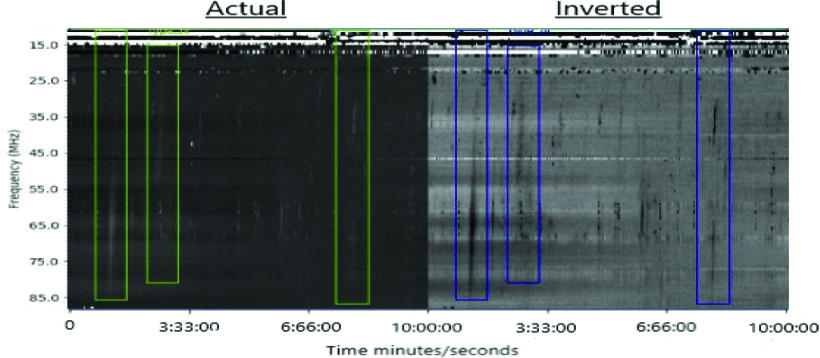
\includegraphics[width=\columnwidth]{scully_yolo.png}
\caption[Automatically detected Type III bursts using YOLO]{Automatically detected Type III bursts using YOLO from \cite{Scully2021}. The colourbar has been inverted in the right panel in order to better display the Type III bursts. }
\label{fig:yolo}
\end{figure}

Implementing this algorithm on REALTA and I-LOFAR would be an ideal test case on real data in real time, especially as we enter into the next solar cycle. Not only this but a detection from the algorithm could be used to trigger a readout off the TBBs too.
In their conclusions, \cite{Scully2021} outline some future developments that could improve their results. In particular, a more physical model of Type III emission is necessary, rather than the simple morphological model presently used.

\subsection{On the Calibration and Interferometric Imaging of Solar Radio Bursts.}
While I at no point doubt the usefulness of imaging algorithms such as CLEAN, the ability to produce different results with the same data and only changing the parameters of the algorithm is too subjective when the main focus of your research is to determine the size of a radio burst. Figure \ref{fig:briggs_comparison} shows how changing the Briggs robustness parameter for weighting the visibilites affects the resulting image. The top panel shows the results for the CLEAN algorithm implemented in WSCLEAN and the bottom panel shows the results when using multiscale cleaning.

\begin{figure}[ht]
\centering
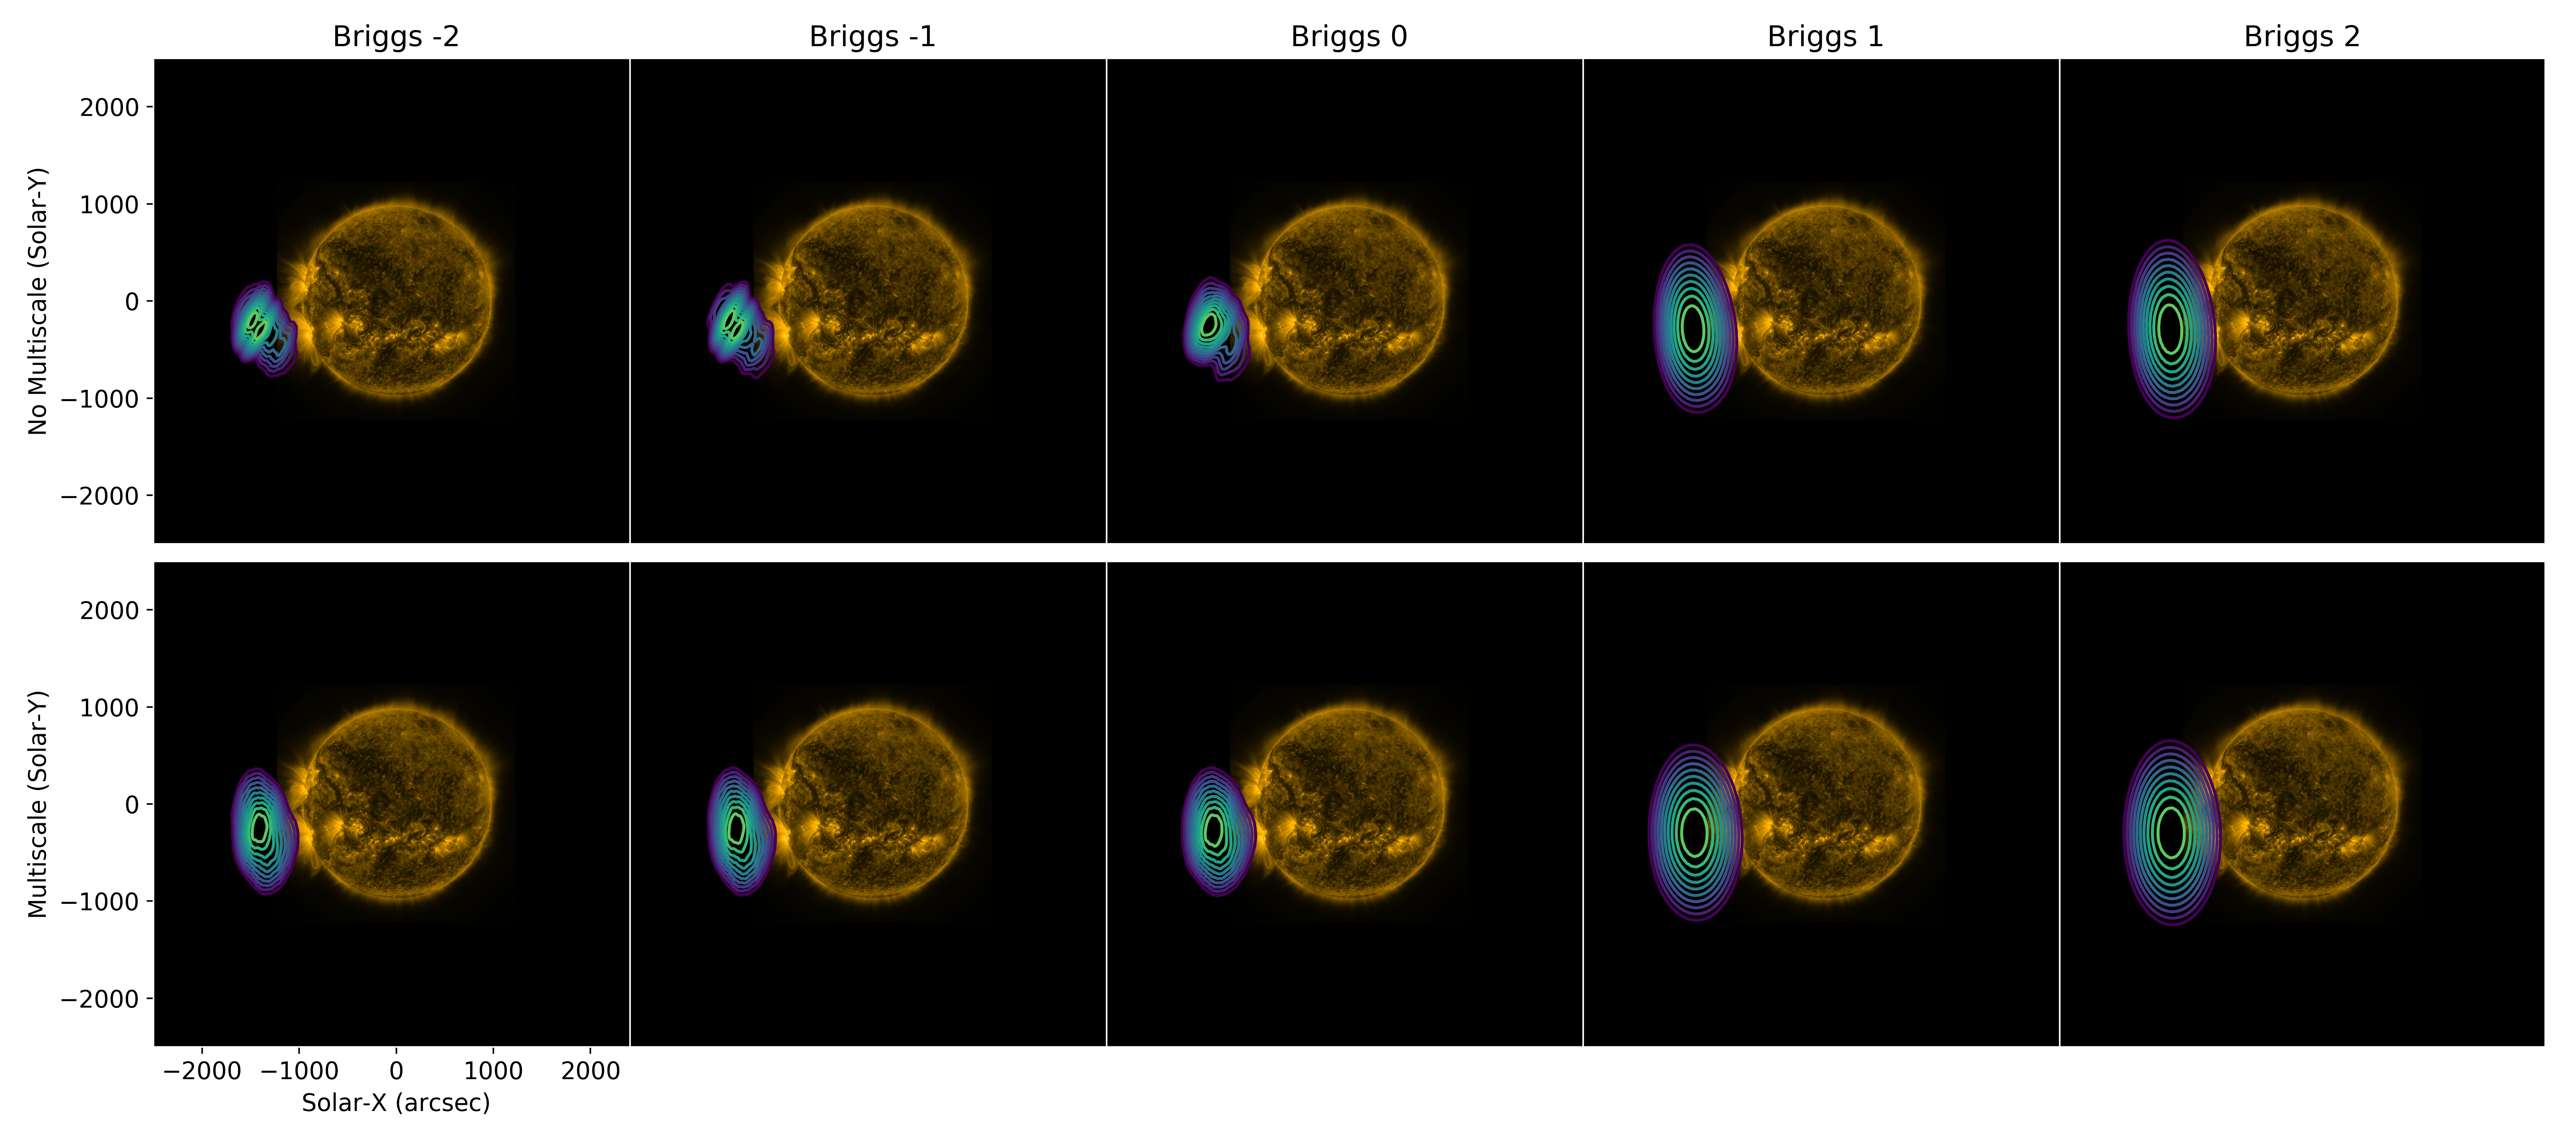
\includegraphics[width=\columnwidth]{briggs_comparison.png}
\caption[An example of the same solar radio burst imaged with different weighting parameters.]{A solar radio burst imaged mulitple times changing the Briggs robustness parameter with (bottom) and without (top) mulitscale cleaning.}
\label{fig:briggs_comparison}
\end{figure}

Interferometric visibilities require calibration in order to account for the effects of the ionosphere. During bursty periods, this calibration can break down and as such more work is needed for a robust calibration procedure for LOFAR. The image in Figure \ref{fig:bad_cal} was made with a bad calibration solution and as such, multiple sources can be seen.

\begin{figure}[ht]
\centering
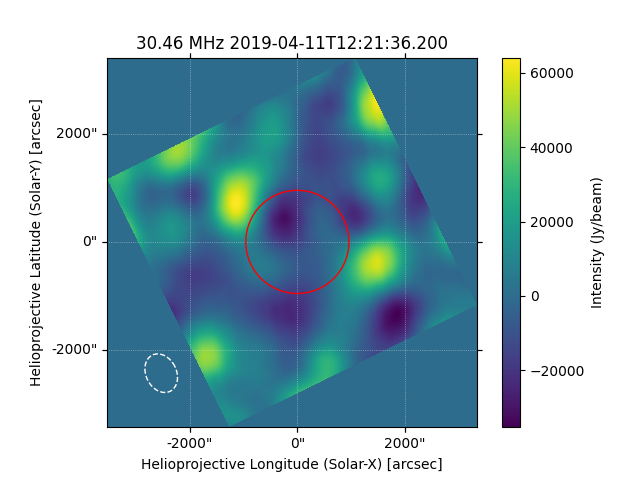
\includegraphics[width=\columnwidth]{2019-04-11T12:21:36.283-image.png}
\caption[An example of a solar radio burst imaged with poor calibration.]{A solar radio burst imaged with poor calibration. The colourbar shows intensity in units of Jy/beam. The red circle indicates the solar limb while the dashed white ellipse is the CLEAN beam.}
\label{fig:bad_cal}
\end{figure}

\subsection{On the Comparisons of Type III and Type IIIb radio bursts}
Type IIIb radio bursts are briefly described in Section \ref{characteristics}. An early theory of the origin of the striations by \cite{Takakura1975} suggests that they are due to an electron beam passing through over dense regions in the solar corona. Recently, \cite{Reid2021} presented simulations and observations of Type IIIb radio bursts where they have determined how the striae fine structure is developed. Beam driven Langmuir wave modulation by turbulence in the solar corona and the spatial motion of these Langmuir waves due to a non-zero group velocity are both necessary in order to match simulations to dynamic spectra and account for individual striation frequency width and duration. Figure \ref{fig:reid_pds} shows the measured and simulated power density spectra for a number of Type IIIb bursts with various background coronas.

\begin{figure}
\centering
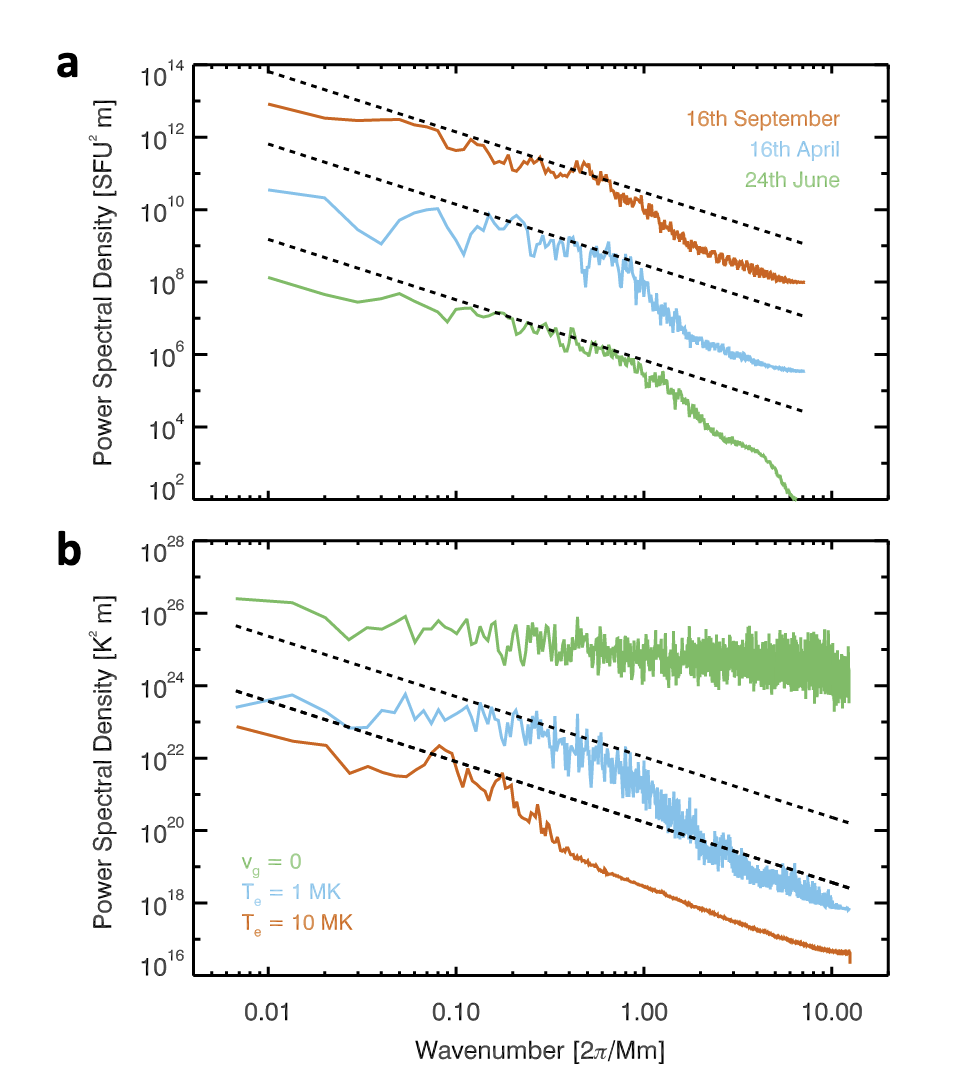
\includegraphics[width=\columnwidth]{reid2021_powerdensityspectra.png}
\caption[Power density spectrum of observed and simulated Type IIIb bursts by \cite{Reid2021}]{Power density spectrum of observed and simulated Type IIIb bursts by \cite{Reid2021}. Panel a shows power density spectra for Type IIIb bursts observed with LOFAR on 16 September 2015 (red), 16 April 2015 (blue) and 24 June 2015 (green). Panel b shows the power density spectra for simulated Type IIIb bursts with a background corona temperature of 1 MK (blue), 10 MK (red) and without a group velocity (green). The dashed balck lines indicate a power law of -5/3, consistent with a Kolmogorov description of turbulence.}
\label{fig:reid_pds}
\end{figure}

Given the effect radio wave scattering has on the size of Type III bursts does not fully agree with scattering simulations (Chapter \ref{chap:observations_vs_theory}), more work is necessary to determine the probable causes of this discrepancy. One possible avenue of investigation would be to perform a similar analysis to Chapter \ref{chap:observations_vs_theory} for Type IIIb bursts. A previous case study of a Type IIIb-III pair (a fundamental-harmonic pair of Type III bursts where the fundamental is a Type IIIb and the harmonic a Type III) was carried out by \cite{Zhang2020}. They found that the fundamental and harmonic emission show different motion as can be seen in Figure \ref{fig:typeIIIbIII} and attribute this to radio wave propagation effects.

\begin{figure}
\centering
\includegraphics[width=\columnwidth]{Zhang_2020.png}
\caption[Type IIIb - III pair observed by \cite{Zhang2020}]{A Type IIIb - III pair observed by \cite{Zhang2020}. Panels a1-3 show the fundamental Type IIIb burst observed with LOFAR and imaged using WSCLEAN. Panels b1-6 show the harmonic Type III burst at a frequency of 26.56 MHz.  }
\label{fig:typeIIIbIII}
\end{figure}

To date there has been no comparison between a large number of Type III and Type IIIb bursts where both are emitting at the fundamental plasma frequency using interferometric observations. Applying a technique similar to the visibility fitting described elsewhere in this thesis to determine a characteristic size could be extremely useful in quantifying the level of turbulence necessary to generate Type IIIb bursts in the first place. This is also an excellent opportunity to use \textit{in-situ} data from PSP and Solar Orbiter to confirm the predictions made with remote measurements from LOFAR and other radio telescopes. 

\section{Concluding Remarks.}
They say science is done incrementally. In that case, this thesis is as incremental as it gets. While I do not claim to have made any ground breaking discoveries, I do truly believe that the work and research undertaken as part of this thesis has improved our understanding of and ability to observe and analyse solar radio emission.  I have but marked the path, it is for others to now follow it.